%!TEX ROOT=main.tex

\section{Domain model}\label{sec:domain-model}

This section will describe entities of the application domain model displayed in figure below.
Some technical information such as data types are omitted for brevity.
Each entity has information about creation date, modification date etc.

\begin{figure}[h]
    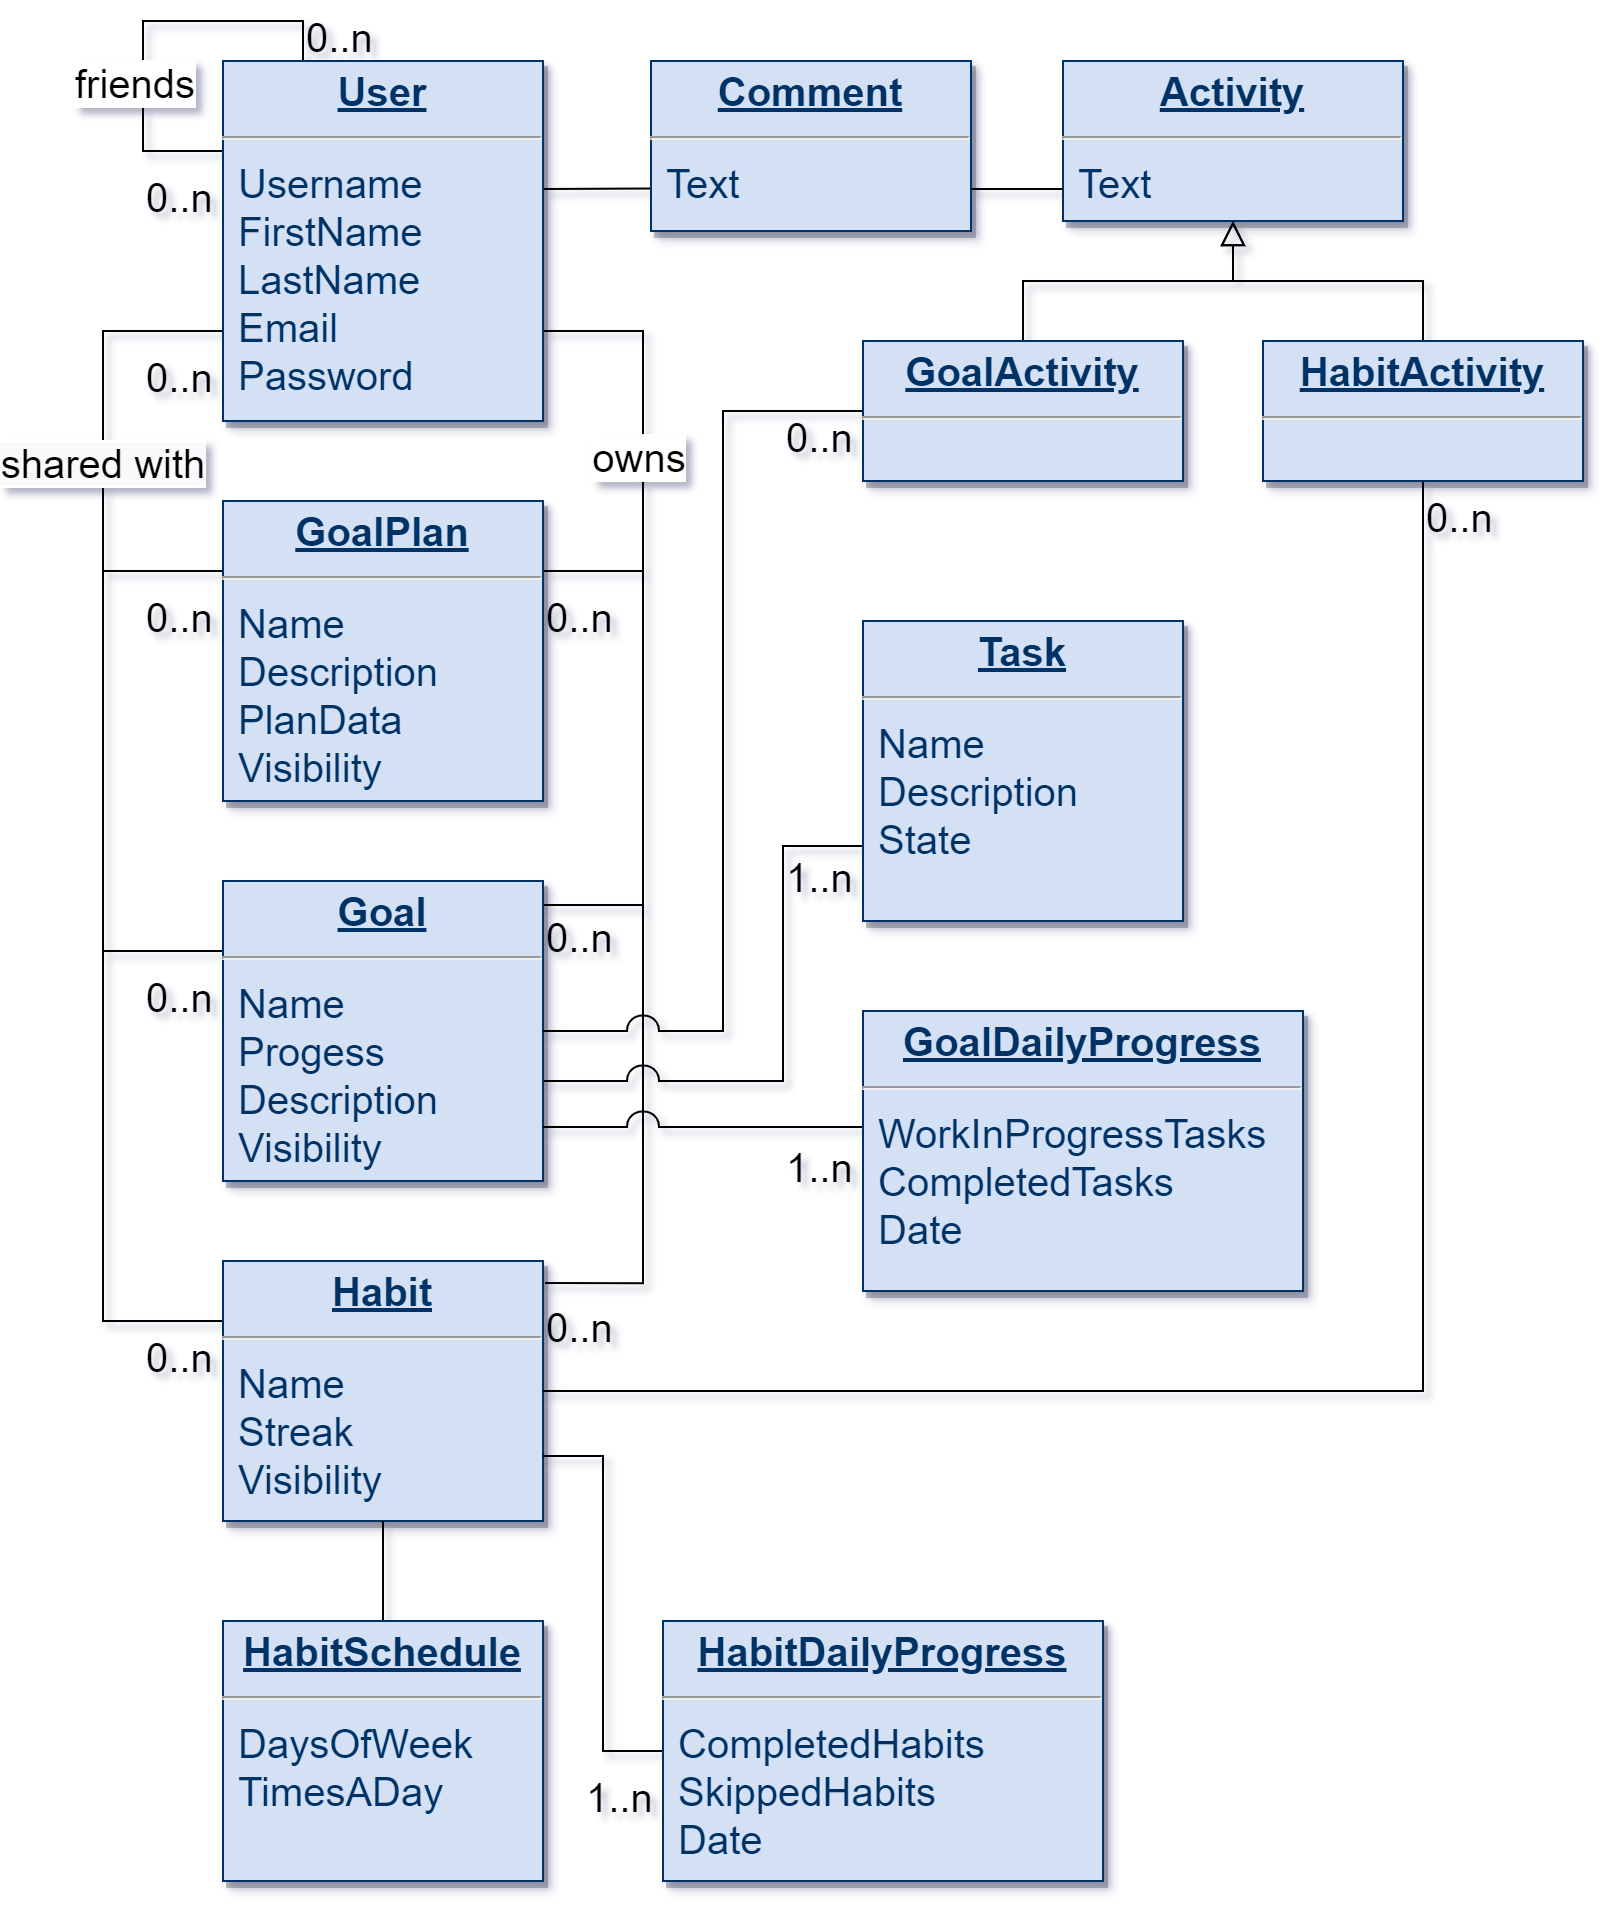
\includegraphics[width=0.75\textwidth]{images/pda-domain-model}
    \caption{Domain model [author]}
    \label{fig:domain-model}
\end{figure}


\subsection{User}\label{subsec:user}

User entity consists of minimum required attributes in order to simplify registration process for end-user.
Recursive relation represents friendship between users, which is required for activity sharing.
Goal plans, goals and habits are always owned by one user and might be shared with other users.
Sharing is used for displaying private plans, goals and habits with specific users.

\subsection{Goal plan}\label{subsec:goal-plan}

Goal plan serves as a blueprint for a goal.
This separation of a plan and a goal allows users to create and to share not only their progress but also plans.
Possible use case would be as follows: a user is proficient in a specific field or skill that others' would like to learn or gain.
They create a goal plan with tasks that contains instructions and share it with any amount of users.
Other users then are able to start a goal pursuing process using this shared plan.

\subsection{Goal}\label{subsec:goal}

Goal is a tool for managing long-term targets.
It is also a specific case of fulfilling a goal plan that is created by user or shared with them.

\subsection{Task}\label{subsec:task}

Task is a building block of a goal.
Task completion used for calculation of a goal's progress.

\subsection{Goal daily progress}\label{subsec:goal-daily-progess}

This entity holds data about daily progress on a specific goal during given day.
It is then used for statistics calculation.

\subsection{Habit}\label{subsec:habit}

Habit is a tool for managing simple and repetitive targets.

\subsection{Habit schedule}\label{subsec:habit-schedule}

Each habit has a schedule.
Initially, it is filled with default values but possible for users to change them.

\subsection{Habit daily progress}\label{subsec:habit-daily-progress}

This entity holds data about daily progress on a specific habit.
It is then used for statistics calculation.

\subsection{Activity}\label{subsec:activity}

This entity holds data about user activities on goals and habits.
When a goal or habit is shared with a user, they will see related activities.

\subsection{Comment}\label{subsec:comment}

It is possible to comment on activities in application and reply to commentaries.
All users with access to activities, can see others' commentaries.